\documentclass[a4paper, numbers=withenddot, 11pt]{scrartcl}

% Vorlage fuer Ausarbeitungen
% Getestet mit pdfTeX; Kodierung: UTF8
% Version 2023-10-13

% Hier Daten eintragen:
\newcommand{\name}{{{Ihr Name}}}
\newcommand{\modulname}{{{Name des Moduls}}}
\newcommand{\thema}{{{Titel der Ausarbeitung}}}
\newcommand{\hochschule}{Fachhochschule Südwestfalen}
\newcommand{\datum}{\today}
% Ende der Daten

\usepackage[utf8]{inputenc}
\usepackage[T1]{fontenc}
\usepackage{lmodern}
\usepackage[ngerman]{babel}
\usepackage[style=alphabetic, backend=biber, bibencoding=utf8]{biblatex}
\addbibresource{literatur.bib}\usepackage{csquotes}
\usepackage{booktabs}
\usepackage{microtype}
\usepackage{graphicx}
\usepackage{scrhack}
\usepackage{setspace}\setstretch{1.1}
\parindent0pt\parskip6pt
\clubpenalty=10000
\widowpenalty=10000
\displaywidowpenalty=10000

\usepackage{listings}
\renewcommand{\lstlistingname}{Listing}
\lstset{basicstyle=\small\ttfamily, breaklines=true, keepspaces=true, columns=fixed}

\title{\thema}
\author{\name\\ \hochschule \\[5mm] Schriftliche Ausarbeitung im Modul\\ „\modulname“}

\begin{document}
% ========== Titel, Inhaltverzeichnis ==========
\maketitle
\tableofcontents

% ========== Hauptteil ==========

\section{Überschrift Ebene eins}

Lorem ipsum dolor sit amet, consetetur sadipscing elitr, sed diam nonumy eirmod tempor invidunt ut labore et dolore magna aliquyam erat, sed diam voluptua. At vero eos et accusam et justo duo dolores et ea rebum. Stet clita kasd gubergren, no sea takimata sanctus est Lorem ipsum dolor sit amet. Lorem ipsum dolor sit amet, consetetur sadipscing elitr, sed diam nonumy eirmod tempor invidunt ut labore et dolore magna aliquyam erat, sed diam voluptua. At vero eos et accusam et justo duo dolores et ea rebum. Stet clita kasd gubergren, no sea takimata sanctus est Lorem ipsum dolor sit amet.

Zitat aus \cite{scheme} und \cite[17]{knuth}. Lorem ipsum dolor sit amet, consetetur sadipscing elitr, sed diam nonumy eirmod tempor invidunt ut labore et dolore magna aliquyam erat, sed diam voluptua. At vero eos et accusam et justo duo dolores et ea rebum.
Es folgt eine Abbildungen. Abbildung \ref{abb_einstein} kann referenziert werden.

\begin{figure}[htbp]
\centering
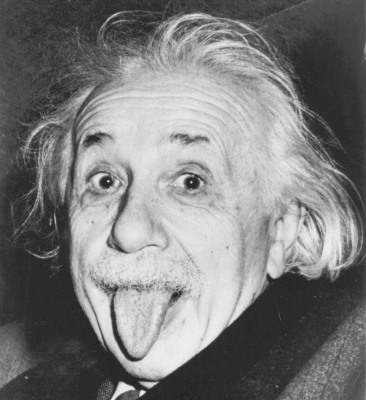
\includegraphics[scale=0.5]{einstein}
\caption{Beschreibung der Abbildung.}
\label{abb_einstein}
\end{figure}

\subsection{Überschrift Ebene zwei}

At vero eos et accusam et justo duo dolores et ea rebum. Stet clita kasd gubergren, no sea takimata sanctus est Lorem ipsum dolor sit amet. Lorem ipsum dolor sit amet, consetetur sadipscing elitr, sed diam nonumy eirmod tempor invidunt ut labore et dolore magna aliquyam erat, sed diam voluptua. At vero eos et accusam et justo duo dolores et ea rebum. Stet clita kasd gubergren, no sea takimata sanctus est Lorem ipsum dolor sit amet. Lorem ipsum dolor sit amet, consetetur sadipscing elitr, sed diam nonumy eirmod tempor invidunt ut labore et dolore magna aliquyam erat, sed diam voluptua.

\section{Aufzählungen, Tabellen und Programmcode}

Eine Aufzählung:

\begin{itemize}
\item Lorem ipsum
\item dolor sit amet
\item consetetur sadipscing elitr
\item sed diam nonumy
\end{itemize}
Eine nummerierte Aufzählung:

\begin{enumerate}
\item Erster Punkt
\item Zweiter Punkt
\item Dritter Punkt
\end{enumerate}
Es folgt Tabelle \ref{beispieltabelle}.

\begin{table}[htbp]
\centering
\begin{tabular}{lrc}
\toprule
Linksbündig & Rechtsbündig & Zentriert \\
\midrule
Lorem &  13 & amet \\
ipsum & 104 & consetetur \\
dolor &   7 & sadipscing \\
sit   &  -5 & elitr \\
\bottomrule
\end{tabular}
\caption{Beschreibung der Tabelle.}
\label{beispieltabelle}
\end{table}

Programmcode im Fließtext: \lstinline{printf("Hello, world!\n");}.
Lorem ipsum dolor sit amet, consetetur sadipscing elitr, sed diam nonumy eirmod tempor invidunt ut labore et dolore magna aliquyam erat, sed diam voluptua. At vero eos et accusam et justo duo dolores et ea rebum. Stet clita kasd gubergren, no sea takimata sanctus est Lorem ipsum dolor sit amet.
Es folgt Programmlisting \ref{beispiellisting}.

\begin{lstlisting}[caption={Beschreibung des Listings.}, label=beispiellisting, frame=tblr, numbers=left]
#include <stdio.h>

int main(void)
{
    printf("Hello, world!\n");
}
\end{lstlisting}
Ein Listing ohne Titel, welches nicht im Listingverzeichnis aufgefühert wird:

\begin{lstlisting}
#include <stdio.h>

int main(void)
{
    printf("Hello, world\n");
}
\end{lstlisting}

Text kann \emph{kursiv} oder \textbf{fett} gesetzt werden.
Lorem ipsum dolor sit amet, consetetur sadipscing elitr, sed diam nonumy eirmod tempor invidunt ut labore et dolore magna aliquyam erat, sed diam voluptua. At vero eos et accusam et justo duo dolores et ea rebum. Stet clita kasd gubergren, no sea takimata sanctus est Lorem ipsum dolor sit amet. Lorem ipsum dolor sit amet, consetetur sadipscing elitr, sed diam nonumy eirmod tempor invidunt ut labore et dolore magna aliquyam erat, sed diam voluptua. At vero eos et accusam et justo duo dolores et ea rebum. Stet clita kasd gubergren, no sea takimata sanctus est Lorem ipsum dolor sit amet.

\chapter{Ein weiteres Kapitel}

Üblicherweise werden Kapitel in separate Dateien ausgelagert und dann mit einem \lstinline{include}-Befehl eingefügt. Das verbessert die Übersichtlichkeit. So wurde diese Datei (\lstinline{mainmatter.tex}) mittels \lstinline!\chapter{Ein weiteres Kapitel}

Üblicherweise werden Kapitel in separate Dateien ausgelagert und dann mit einem \lstinline{include}-Befehl eingefügt. Das verbessert die Übersichtlichkeit. So wurde diese Datei (\lstinline{mainmatter.tex}) mittels \lstinline!\chapter{Ein weiteres Kapitel}

Üblicherweise werden Kapitel in separate Dateien ausgelagert und dann mit einem \lstinline{include}-Befehl eingefügt. Das verbessert die Übersichtlichkeit. So wurde diese Datei (\lstinline{mainmatter.tex}) mittels \lstinline!\include{mainmatter}! eingefügt.
! eingefügt.
! eingefügt.


% ========== Literaturverzeichnis ==========
\printbibliography
\chapter*{Erklärung}

Ich erkläre hiermit, dass ich die vorliegende Arbeit selbstständig verfasst und dabei keine anderen als die angegebenen Hilfsmittel benutzt habe. Sämtliche Stellen der Arbeit, die im Wortlaut oder dem Sinn nach Werken anderer Autoren entnommen sind, habe ich als solche kenntlich gemacht. Die Arbeit wurde bisher weder gesamt noch in Teilen einer anderen Prüfungsbehörde vorgelegt und auch noch nicht veröffentlicht.

\bigskip
\noindent
\datum

\vspace{25mm}

\noindent
\name

\end{document}
